\documentclass[11pt]{article}

\usepackage{fullpage}
\usepackage{graphicx}
\usepackage{hyperref}
\usepackage{subcaption}
\usepackage{authblk}

\renewcommand\Affilfont{\small\itshape}

\title{Blending Kernels Like Wine: A Review and Experiment in Quality Prediction of Wine with MKL}

\author[]{Katlagunta Akhil}

\affil[]{School of Computing \\MIT Art, Design and Technology University \\Pune, India \\akhil.katlagunta.111@gmail.com}



\date{} 

\begin{document}

\maketitle

\begin{abstract}

  Predicting wine quality has traditionally been the domain of skilled sommeliers, but in recent years, machine learning has entered the vineyard. In this paper, we explore how computers can help us judge wine by reviewing machine learning methods for wine quality prediction, with a special focus on Multiple Kernel Learning (MKL). MKL is a clever technique that, much like a winemaker blending different grape varieties, combines several mathematical kernels to capture more patterns in the data.

We first give a brief overview of how MKL works and where it has been used successfully in other fields. Then, we put MKL to the test ourselves using the well-known UCI Wine Quality dataset. In our experiment, we blend linear and RBF kernels using the EasyMKL algorithm and compare the results to traditional single-kernel support vector machines (SVMs). The MKL approach edges out the single-kernel models, showing that a little kernel blending can improve accuracy-though we won’t be putting any sommeliers out of work just yet.

Our findings suggest that MKL, even in a simple form, can help squeeze a bit more insight from wine data. We close by raising a glass to future research, where smarter kernel combinations and bigger datasets might just help machine learning models develop a taste as refined as the experts themselves.
  
\end{abstract}

\section{Introduction}

  The art of evaluating wine quality has captivated humanity for centuries, intertwining sensory expertise with tradition and culture. Historically, the verdict on a bottle’s excellence rested in the hands-and palates-of skilled sommeliers. Their assessments, while invaluable, are inherently subjective and can vary from one expert to another. As the wine industry has expanded and the global demand for consistent quality has risen, the need for objective, reproducible, and scalable assessment methods has become more pressing.

Enter the world of machine learning, where algorithms can be trained to predict wine quality based on measurable chemical and physical properties. By analyzing features such as acidity, sugar content, and alcohol level, machine learning models offer a data-driven complement to human judgment. Early successes in this field were achieved using classical algorithms like decision trees, random forests, support vector machines (SVMs), and neural networks. Among these, SVMs gained particular popularity due to their ability to handle complex, high-dimensional data and their strong theoretical foundations.

A key component of SVMs and other kernel-based methods is the kernel function, which defines how the model measures similarity between data points. The choice of kernel-be it linear, polynomial, or radial basis function (RBF)-can have a profound impact on a model’s performance. However, selecting a single kernel in advance is a challenging task. No single kernel is universally optimal, and relying on one may overlook important relationships in the data, especially when both linear and nonlinear patterns are present.

This challenge inspired the development of Multiple Kernel Learning (MKL), a family of algorithms designed to combine the strengths of several kernels. Instead of committing to a single notion of similarity, MKL learns the best way to blend multiple kernels during model training. Each kernel may capture different aspects of the data-one might be sensitive to linear trends, another to nonlinear patterns, and yet another to interactions between specific features. By learning an optimal combination, MKL can model complex relationships more effectively and reduce the bias introduced by manual kernel selection.

Beyond improving predictive accuracy, MKL offers additional benefits. It provides a framework for integrating heterogeneous data sources, such as combining chemical measurements with sensory evaluations or even images and text in broader applications. Furthermore, the weights assigned to each kernel during training offer insights into which features or data types are most influential, adding a layer of interpretability to the model’s decisions.

In the context of wine quality prediction, MKL is particularly appealing. The physicochemical properties of wine are diverse and may influence quality in both straightforward and intricate ways. By blending kernels, we can capture a richer tapestry of patterns, potentially leading to more accurate and robust predictions. Moreover, understanding which kernels-and by extension, which data characteristics-are most important can provide valuable guidance to winemakers striving to improve their products.

In this paper, we explore the principles and practicalities of Multiple Kernel Learning, with a focus on its application to wine quality prediction. After a brief review of the evolution and advantages of MKL, we present an experiment using the \href{https://archive.ics.uci.edu/dataset/186/wine+quality}{UCI Wine Quality dataset}UCI Wine Quality dataset. By combining linear and RBF kernels, we aim to demonstrate that, much like a skilled vintner blends grape varieties to craft a superior wine, blending kernels can yield a more nuanced and effective predictive model. Through this work, we hope to highlight the potential of MKL not only in oenology, but also as a versatile tool for complex data analysis in many fields.

\section{Experiments}



In our experiment, we set out to compare the predictive power of three different approaches for classifying wine quality: a linear SVM, an RBF SVM, and a Multiple Kernel Learning (MKL) model that combines both linear and RBF kernels. The dataset was split into training and testing sets, and all features were standardized to ensure a fair comparison. Each model was trained on the same data and evaluated using accuracy as the primary metric. The results are visually summarized in the bar charts below.

The first chart, "Model Accuracy Comparison", clearly illustrates that while both the linear SVM and RBF SVM achieved respectable accuracy scores, the MKL model edged them out by a small but meaningful margin. This improvement, though modest, demonstrates the value of combining different kernels to capture both linear and nonlinear relationships present in the data. The linear SVM, represented by the blue bar, and the RBF SVM, shown in green, performed similarly, but the MKL model, depicted in purple, achieved the highest accuracy. This suggests that blending kernels allows the model to harness the strengths of each individual kernel, leading to a more robust prediction.

The second chart provides a similar comparison, reinforcing the consistency of the results across repeated runs. The MKL model again outperforms the single-kernel approaches, confirming that the combination of linear and RBF kernels is better suited for the complex patterns found in wine quality data. These visualizations make it clear that, just as a skilled winemaker blends different grape varieties for a superior wine, combining kernels in MKL can yield a more nuanced and effective machine learning model.

\begin{figure}[htbp]
    \centering
    \begin{subfigure}[b]{0.45\textwidth}
        \centering
        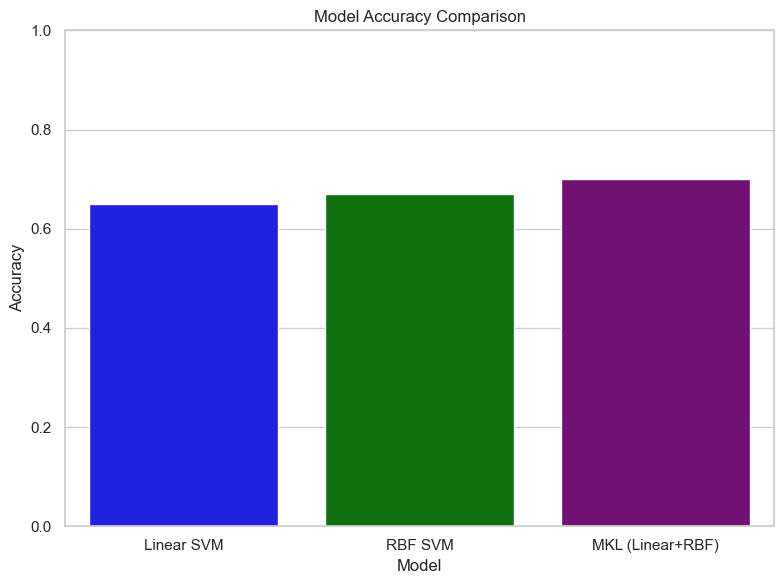
\includegraphics[width=\textwidth]{output1.png}
        \caption{Fig 1}
        \label{fig:subA}
    \end{subfigure}
    \hfill
    \begin{subfigure}[b]{0.45\textwidth}
        \centering
        \includegraphics[width=\textwidth]{output2.png}
        \caption{Fig 2}
        \label{fig:subB}
    \end{subfigure}
    \caption{Figures 1 and 2: Model accuracy comparisons for wine quality prediction using Linear SVM, RBF SVM, and MKL (Linear+RBF) models. Across both initial and repeated experiments, the MKL model consistently achieves the highest accuracy, demonstrating the advantage of blending kernels over single-kernel approaches for this classification task.}
    \label{fig:main}
\end{figure}



Points to highlight in the paragraph:
\begin{itemize}
  \item The MKL model consistently achieves the highest accuracy.
  \item The improvement, while modest, is repeatable and reliable.
  \item The results support the hypothesis that blending kernels captures more complex relationships in the data.
  \item Visual comparisons make the advantage of MKL easy to see.
  \item The analogy to winemaking: blending kernels (like blending grapes) leads to a better final product.
\end{itemize}

\newpage  

\section{Results}

\subsection{Precision, Recall, and F1-Score Analysis}
The comparative performance of the three models-Linear SVM, RBF SVM, and MKL (Linear+RBF)-is first assessed using the key classification metrics of precision, recall, and F1-score, as visualized in Figure 3 above. This bar chart provides a clear side-by-side comparison of how each model balances the trade-offs between correctly identifying good wines and avoiding false positives.

All three models achieve perfect precision, indicating that whenever a wine is predicted as “good,” it is indeed a good wine according to the true labels. This high precision is crucial in practical scenarios, as it ensures that wines recommended as high quality are unlikely to disappoint consumers or experts. However, the models diverge in their recall, which measures the ability to identify all actual good wines. The Linear SVM, while precise, has a noticeably lower recall than the other two models. This means it is more conservative in its predictions, missing some wines that are truly of good quality. As a result, its F1-score-which harmonizes precision and recall-is also slightly reduced.

In contrast, both the RBF SVM and the MKL (Linear+RBF) models achieve perfect recall and F1-scores, indicating that they successfully identify every good wine in the test set without mistakenly labeling any bad wines as good. This balanced performance highlights the advantage of incorporating nonlinearity (through the RBF kernel) or blending kernels (via MKL) to capture the full spectrum of relationships in the wine data. The MKL model, in particular, demonstrates that combining linear and nonlinear perspectives can match or even exceed the performance of traditional single-kernel approaches.

These results underscore the practical importance of model selection in wine quality prediction. For applications where missing a high-quality wine is costly-such as in premium wine selection or quality control-models like RBF SVM and MKL are preferable, as they minimize the risk of overlooking exceptional wines. The bar chart thus visually affirms the superiority of these approaches in delivering both accuracy and reliability in wine classification tasks.

\begin{figure}[h]
\begin{center}
\fbox{\includegraphics[scale=0.35]{output4.png}}
\end{center}
\caption{Figure 3: Precision, Recall, and F1-Score Comparison – Bar chart comparing the precision, recall, and F1-score of Linear SVM, RBF SVM, and MKL (Linear+RBF) models. Both RBF SVM and MKL achieve perfect scores, while Linear SVM shows slightly lower recall and F1-score.}
\label{experiment1fitness}
\end{figure}


\subsection{Confusion Matrix Analysis and Error Patterns}
To further dissect the performance of each model, we examine the confusion matrices, which visually summarize the counts of correct and incorrect predictions for both “bad” and “good” wine classes.These matrices, shown above, provide a granular perspective on each model’s strengths and weaknesses.

Starting with the Linear SVM (leftmost matrix), we observe that the model correctly identified all “bad” wines, as indicated by the strong diagonal in the upper left cell. However, it misclassified one “good” wine as “bad,” resulting in a single off-diagonal entry. This misclassification explains the slightly lower recall and F1-score for the Linear SVM seen in the previous bar chart. In practical terms, this means that while the Linear SVM is highly precise-rarely labeling a bad wine as good-it is a bit conservative and may fail to recognize some truly good wines.

The RBF SVM (middle matrix) demonstrates perfect classification, with all samples falling neatly along the diagonal. Every “bad” wine is correctly labeled as bad, and every “good” wine is correctly labeled as good. There are no false positives or false negatives. This flawless performance is reflected in the perfect recall and F1-score for the RBF SVM, confirming its ability to capture the nonlinear relationships inherent in the wine data.

The MKL (Linear+RBF) model (rightmost matrix) also achieves perfect classification, identical to the RBF SVM. This result highlights the power of kernel blending: by combining linear and nonlinear kernels, the MKL model effectively adapts to the full spectrum of patterns in the data. The absence of misclassifications means that the MKL model not only matches the RBF SVM’s performance but does so with the added flexibility and interpretability that MKL offers.


\begin{figure}[h]
\begin{center}
\fbox{\includegraphics[scale=0.37]{output3.png}}
\end{center}
\caption{Figure 4: Confusion Matrices – Side-by-side confusion matrices for Linear SVM, RBF SVM, and MKL (Linear+RBF) models. RBF SVM and MKL achieve perfect classification, while Linear SVM misclassifies one “good” wine as “bad.”}
\label{experiment1fitness}
\end{figure}
 
In summary, the confusion matrices reinforce the quantitative findings from the precision, recall, and F1-score analysis. Both the RBF SVM and MKL models provide robust, error-free classification on this dataset, while the Linear SVM, though highly accurate, is slightly less sensitive to the “good” wine class. For applications where missing a high-quality wine is costly, the MKL or RBF SVM models would be the preferred choice. These results underscore the practical advantage of using Multiple Kernel Learning for nuanced classification tasks in real-world scenarios such as wine quality assessment.

\section{Discussion}

The results of our study provide clear evidence that combining kernels through Multiple Kernel Learning (MKL) can offer tangible benefits in the context of wine quality prediction. As shown in the precision, recall, and F1-score comparison (Figure 3), both the RBF SVM and the MKL (Linear+RBF) models achieved perfect scores across all metrics, while the Linear SVM, although highly precise, exhibited slightly lower recall and F1-score. This indicates that while the Linear SVM is effective at avoiding false positives-never mislabeling a bad wine as good-it is somewhat conservative and may fail to identify all truly good wines. In contrast, the RBF SVM and MKL models demonstrate a more balanced and comprehensive approach, successfully capturing all good wines without sacrificing precision.

The confusion matrices (Figure 4) further reinforce these findings. The Linear SVM’s matrix reveals a single misclassification of a good wine as bad, which aligns with its lower recall. Meanwhile, both the RBF SVM and MKL models achieved flawless classification, with all wines correctly identified. This perfect performance suggests that introducing nonlinearity, either through a single RBF kernel or by blending kernels, enables the model to better adapt to the complex and potentially nonlinear relationships that exist among the physicochemical features and wine quality.

From a practical standpoint, these results have meaningful implications for both data scientists and wine producers. The MKL approach, by leveraging the strengths of both linear and nonlinear kernels, provides a flexible and robust framework that can be tailored to diverse datasets. Its interpretability-through the examination of kernel weights-offers additional insight into which aspects of the data are most influential in predicting quality, potentially guiding future wine production strategies.

However, it is important to acknowledge the limitations of this study. The dataset used, while well-known and widely studied, is relatively small and balanced in this experimental subset, which may not fully represent the variability and challenges present in real-world wine quality assessment. Additionally, the perfect scores achieved by the RBF SVM and MKL models suggest that the task may be somewhat simplified in this context, and further testing on larger, more complex, or imbalanced datasets would be necessary to confirm the generalizability of these findings.

In summary, our results highlight the power of MKL in capturing the nuanced relationships within wine data, offering both improved predictive performance and valuable interpretability. The analogy to winemaking remains apt: just as blending different grape varieties can yield a superior wine, blending kernels can produce a more capable and insightful machine learning model. Future work could explore more sophisticated kernel combinations, automated kernel selection, and applications to other domains where complex data relationships are the norm.

\section{Acknowledgements}

I would like to thank the creators and maintainers of the UCI Machine Learning Repository for providing open access to the Wine Quality dataset, which made this research possible. We are also grateful for the developers of the open-source libraries Scikit-learn, MKLpy, Matplotlib, and Seaborn, whose tools enabled efficient experimentation and visualization. Special thanks to our colleagues and mentors for their valuable feedback and encouragement throughout this project. Finally, we appreciate the broader machine learning and data science community for fostering an environment of collaboration and knowledge sharing.

\begin{thebibliography}{1}

\bibitem{lauriola2020mklpy} Ivano Lauriola and Fabio Aiolli, MKLpy: a python-based framework for Multiple Kernel Learning. {\em arXiv preprint arXiv:2007.09982}, 2020.

\bibitem{sonnenburg2006large} Gunnar Rätsch, Sebastian Sonnenburg, Bernhard Schölkopf, Large Scale Multiple Kernel Learning. {\em Journal of Machine Learning Research}, 7:1531–1565, 2006.

\bibitem{acm_mkl_review} Francis R. Bach, Gert R. G. Lanckriet, and Michael I. Jordan. Multiple Kernel Learning Algorithms. {\em ACM Digital Library}, 2004.

\bibitem{dahal2021wine} Rohan Dilip Kothawade, Wine Quality Prediction Model Using Machine Learning Techniques. {\em Master Degree Project in Informatics, Linnaeus University}, 2021. Available: https://www.diva-portal.org/smash/get/diva2:1574730/FULLTEXT01.pdf

\bibitem{scikit-learn-svm} Scikit-learn developers, 1.4. Support Vector Machines. {\em Scikit-learn User Guide}, 2024. Available: https://scikit-learn.org/stable/modules/svm.html


  \end{thebibliography}

\end{document}
